\chapter{METODOLOGIA}
\label{cap:metodologia}

Este capítulo descreve a metodologia e as técnicas que serão empregados na pesquisa e desenvolvimento do sistema proposto, destacando as tecnologias e dispositivos necessários.

\section{Visão geral do sistema proposto}

O Sistema de Identificação de Condutores baseado em Técnicas de Inteligência Computacional terá a função de efetuar a identificação do condutor que dirige o veículo e detectar possíveis situações de roubo e furto do mesmo. Para tal, a identificação será feita por meio do reconhecimento de certos padrões de direção característicos de cada condutor. Isto é possível através da coleta de dados provenientes do barramento de comunicação do veículo, por meio da interface OBD-II e coletados pelo dispositivo de leitura ELM327, que transmite via \textit{bluetooth} para o \textit{smartphone} a ele conectado, que também fornece dados referentes à dinâmica de direção.

Antes de submeter os dados no algoritmo de identificação, será efetuado um processamento e fusão destes dados, de modo a remover ruídos e possíveis \textit{outliars}, além de melhorar a extração de características pelo sistema. Feito isso, dentro do grupo de condutores de cada \textit{dataset}, será determinado um conjunto de condutores autorizados, treinando o modelo computacional com as características destes. Após o treinamento, serão efetuados testes com dados de direção desconhecidos pelo modelo, de forma a avaliar o desempenho do mesmo. Esta validação será utilizada para comprovar a viabilidade do sistema de identificação de condutores. A Figura~\ref{fig:flux} apresenta graficamente o sistema e os passos até a identificação.

\begin{figure}[!htb]
\centering
\caption{Visão geral do Sistema de Identificação de Condutores baseado em Técnicas de Inteligência Computacional.} %legenda
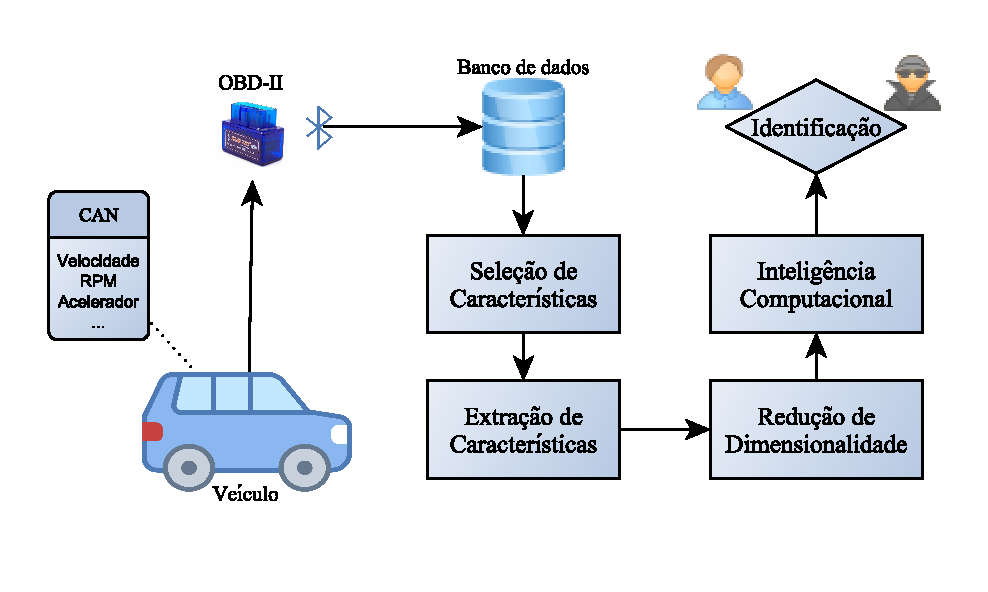
\includegraphics[width=0.7\linewidth]{FLUXOGRAMA.eps}\\ 
{\small Fonte: Próprio autor.} %Fonte da imagem
\label{fig:flux} %rotulo para refencia
\end{figure}

Uma vez determinada a viabilidade da identificação de condutores por meio dos modelos implementados, será desenvolvido um sistema evolutivo, que poderá ser implementado em aplicações reais. Este modelo terá como objetivo aprimorar seu sistema de classificação através do uso contínuo de dados de direção gerados pelos condutores autorizados, uma vez que o estilo de direção poderá ser alterado por uma série de fatores, como horário, questões climáticas (chuva, neblina, entre outros) e emocionais do condutor.

A Figura~\ref{fig:flux2} apresenta o esquema de operação deste sistema. No modelo computacional evolutivo já está incluso as técnicas de seleção e extração de características, bem como as de redução de dimensionalidade (caso necessário). O principal motivo para a implementação de um modelo de aprendizado \textit{online} é justamente a necessidade do modelo estar sempre se aprimorando, baseado no fluxo de dados de direção que constantemente o alimentará. A ideia é que a tarefa de classificação seja sempre a mais precisa possível e que se adapte aos mais diferentes estilos de direção de cada condutor autorizado.


\begin{figure}[!htb]
	\centering
	\caption{Visão geral do Sistema de Identificação de Condutores baseado em Técnicas de Inteligência Computacional.} %legenda
	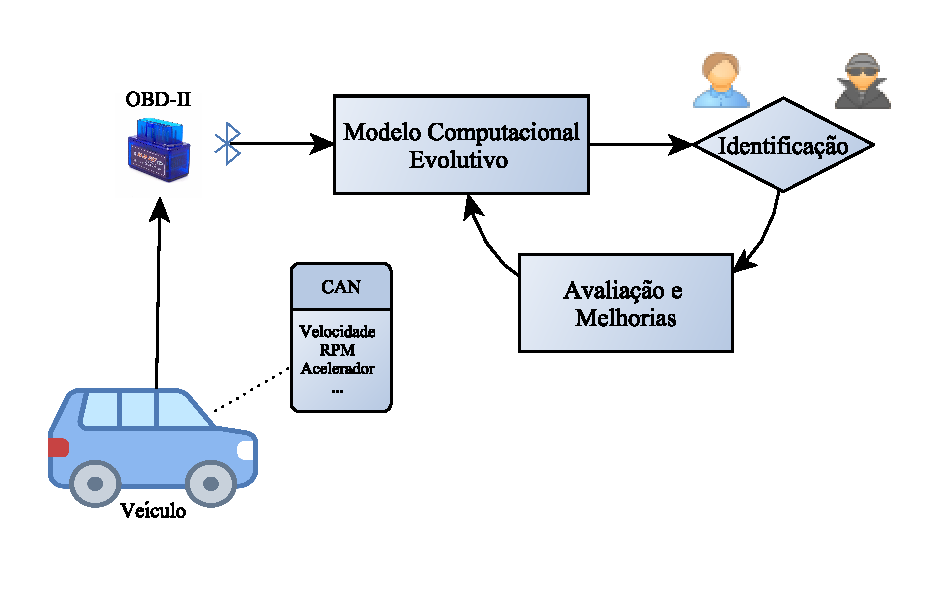
\includegraphics[width=0.7\linewidth]{FLUX_parte2.eps}\\ 
	{\small Fonte: Próprio autor.} %Fonte da imagem
	\label{fig:flux2} %rotulo para refencia
\end{figure}


\section{\textit{Datasets} Utilizados}

No desenvolvimento preliminar do sistema proposto foi utilizado o \textit{dataset} disponibilizado por \citeonline{kwak2016know}, juntamente com o \textit{Hacking and Countermeasure Research Lab}\footnote[1]{http://ocslab.hksecurity.net}. Este \textit{dataset} consiste em dados extraídos do barramento CAN do veículo, coletados por por meio da interface \textit{On Board Diagnostics 2} (OBD-II) do veiculo e do \textit{scanner} CarbigsP. O veículo usado na coleta dos dados (Kia Soul) possui diversos sensores e atuadores que fornecem um montante representativo de dados que podem ser usados para detectar certos padrões inerentes ao comportamento do condutor e até mesmo sua identidade. Estes dados foram amostrados em uma frequência de 1Hz com 51 sensores medidos.

Na coleta de dados, dez indivíduos conduziram o veículo em quatro rotas distintas em Seul, Coreia do Sul. Os autores consideraram três categorias de vias: urbano, rodovia e estacionamento. Cada condutor foi submetido a duas sessões de direção que passa por todos os tipos de vias, totalizando 23 km.

A grande vantagem desde conjunto de dados em comparação à outros utilizados em abordagens similares é que este \textit{dataset} é mais recente, colhido a partir de julho de 2015, e mais completo uma vez que veículos mais novos possuem maior quantidade de sensores embarcados. Outra vantagem relevante do mesmo é a preocupação que os autores tiveram em relação à confiabilidade dos dados, visto que os experimentos foram conduzidos em situações similares, como o fator temporal (entre 8 da manhã e 11 da noite em dias de semana) e duas viagens diferentes para cada condutor, aumentando a extração de traços característicos de direção de cada condutor, e portanto, proporcionando uma classificação de condutores mais eficiente. O conjunto de dados fornecidos tem um total de 94.401 amostradas a 1Hz, com tamanho total de 16,7Mb.

Em testes futuros também será considerado o uso do \textit{dataset} UYANIK, cordialmente cedido pelo VPALAB da Universidade de Sabanci (Istambul, Turquia) \cite{Abut2007}. Este \textit{dataset} contém dados de um grande número de condutores colhidos a partir de dados do barramento CAN, sensores inerciais e GPS e é amplamente utilizado em diversos trabalhos que envolvem identificação de condutores \cite{Martinez2016a} \cite{jafarnejad2017} \cite{DelCampo2014}. Estes dados servirão para avaliar a aptidão das técnicas de processamento de dados e de inteligência computacional, de modo a se determinar as que melhores se encaixam na tarefa de identificação e autenticação dos condutores. Entre as vantagens deste conjunto de dados é o fato de, além dos dados do barramento CAN, estar presente dados obtidos a partir de sensores inerciais (tal qual encontrado nos \textit{smartphones} atuais), que proporcionam informações mais completas relacionadas à dinâmica de direção.

Outro \textit{dataset} que poderá ser utilizado é o \textit{Driving Behavior Dataset} do LAC (\textit{Laboratory for Advanced Collacoration})\footnote[1]{http://www.inf.puc-rio.br/~rvasconcelos/DataSet/dataset.html} da PUC-Rio, sendo este o único banco de dados de condução brasileiro~\cite{OLIVEIRAVASCONCELOS2017}. O veículo utilizado foi a versão brasileira do Citröen C3, equipado com um \textit{smartphone} conectado à um dispositivo OBD-II via \textit{bluetooth}. Foram selecionados 25 motoristas para a coleta dos dados, sendo dezesseis  do sexo masculino e nove do sexo feminino, com idade variando de 20 a 60 anos. Os motoristas possuíam de 2 a 42 anos de experiência. Além dos dados do OBD-II, foram aproveitados os sensores embarcados no \textit{smartphone}, sendo estes: acelerômetro, GPS, giroscópio e orientação (bússula). Foi definido um percurso pavimentado em Aracaju-SE totalizando aproximadamente 14.5 Km, cujas ruas e avenidas possuíam de uma a três faixas. Além disso, a rota contém rotatórias, semáforos, faixa de pedestres, cruzamentos, interseções (parada total) e curvas de aproximadamente 45$^\circ$ e 90$^\circ$. O limite de velocidade em todo o percurso é de 60 Km/h.

\section{Desenvolvimento Preliminar}

Com o objetivo de analisar e comprovar a viabilidade do sistema proposto, foram elaborados uma série de experimentos preliminares, analisando diversas técnicas de seleção e extração de características, bem como diferentes algoritmos de classificação. Dentre os \textit{datasets} supracitados, foi utilizado o fornecido pelo \textit{Hacking and Countermeasure Research Lab}.

\subsection{Seleção de Características}

O conjunto de dados é dividido em dez condutores numerados entre 0 e 9. Porém o objetivo do trabalho é classificar os condutores entre não autorizado e autorizado. Para tal, foram selecionados aleatoriamente três condutores que foram definidos como autorizados (classe 1), como membros de uma mesma família ou empresa que compartilham o mesmo veículo, e restante dos condutores foram definidos como não autorizados (classe 0). 

A implementação do sistema de testes passa inicialmente pela seleção de quais características disponíveis no conjunto de dados colhidos no barramento CAN serão utilizadas na tarefa de identificação dos condutores. Neste estágio, foi utilizado a técnica FDA, implementado para Python por \citeonline{li2016feature} especialmente para seleção de características para classificadores. Foram selecionadas oito características de entrada de maior relevância, as quais são descritas na Tabela~\ref{tab:var}.

\begin{table}[h]
	\centering
	\caption{Características de entrada selecionadas.}
	\label{tab:var}
	\begin{tabular}{cc}
		\hline
		Característica & Descrição \\ \hline
		1 & Valor do pedal de acelerador \\
		2 & Ângulo de esterçamento do volante \\
		3 & Velocidade do Veículo \\
		4 & Velocidade do Motor \\
		5 & Abertura da Válvula reguladora \\
		6 & Aceleração Longitudinal \\
		7 & Aceleração Lateral \\
		8 & Pressão do ar de entrada \\ \hline
	\end{tabular}
\end{table}

\subsection{Extração de Características}

De posse destas variáveis, passa-se agora ao estágio de extração de características de forma a minimizar os efeitos de flutuação dos valores e caracterizar a distribuição de características efetivamente. Além dos valores de cumulantes em atraso zero (variância (segunda ordem), assimetria (terceira ordem) e curtose (quarta ordem)), foram utilizados os valores de mediana e média, totalizando assim cinco características estatísticas por variável.

Estas estatísticas foram obtidas por meio de certo período de amostragem determinadas por meio de um janelamento temporal. De forma a também determinar qual o intervalo de tempo de janelamento é mais adequado para a tarefa de identificação dos condutores, foram testadas janelas de 15, 30, 60, 90 e 120 segundos. 

\subsection{Redução da Dimensionalidade}

Pode-se observar que no estágio de extração de características estatística, de cada variável de entrada são derivados cinco elementos, totalizando quarenta variáveis de entrada. Esta quantidade de valores dificulta o desempenho do classificador em termos de eficiência computacional e até comprometer a capacidade de generalização do mesmo. Sendo assim, mais uma vez foi aplicado o Discriminante de Fisher de forma a selecionar destas quarenta varáveis derivadas as dez mais significantes para a tarefa de classificação.

Ainda com a redução obtida no passo anterior, o número de variáveis de entrada pode dificultar o desempenho do classificador. Para contornar esta situação, foram adotados métodos de redução de dimensionalidade de forma a reduzir o espaço de entrada de dez variáveis para somente quatro, sem que ocorram perdas de características significativas. As técnicas testadas são as de Análise de Componentes Principais (PCA), Análise de Componentes Principais Incrementais (IPCA) e Análise de Componentes Independentes (ICA), todos considerando quatro componentes. Portanto o espaço de dez variáveis oriundos da seleção por meio do Discriminante de Fisher foi reduzido a um espaço de apenas quatro componentes no classificador.

\subsection{Classificação}

Para a tarefa de identificação dos condutores foram considerados três algoritmos de classificação distintos. Os algoritmos foram implementados em Python utilizando a biblioteca \textit{scikit-learn - Machine Learning in Python} \cite{scikit-learn}. Os classificadores foram configurados de acordo com os seguintes parâmetros:

\begin{itemize}
	\item K – \textit{Nearest Neighbor} (KNN): número de vizinhos: 3; pesos uniformes.
	
	\item \textit{Random Forest} (RF): 50 estimadores; profundidade máxima: 10; amostras mínimas por folha: 10.
	
	\item Redes Neurais Artificiais (MLP): Número de camadas escondidas = 2, número de neurônios por camada = 10, máximo de épocas de treinamento = 500.
	
\end{itemize}

\subsection{Configuração dos experimentos}

Os experimentos foram conduzidos de forma a testar todas as combinações de técnicas possíveis de forma a se conseguir  o maior número de acertos na identificação dos condutores. Estas combinações envolvem as cinco janelas temporais (15, 30, 60, 90 e 120 segundos), três técnicas de redução de dimensionalidade (PCA, IPCA e ICA) e três classificadores (KNN, RF e MLP). A combinação destes elementos totalizam quarenta e cinco cenários diferentes. Cada classificador é treinado e testado dez vezes e cada uma destas é efetuada a separação entre dados de treino (80\%) e teste (20\%). Em cada um dos testes é feita uma permutação aleatória dos dados, de forma a não comprometer a capacidade de generalização do classificador.

O objetivo final dos testes é maximizar a taxa de acertos entre os condutores autorizados (classe 1) e não autorizados (classe 0). O fluxo geral dos experimentos é descrito na Figura~\ref{fig:fluxo}.

\begin{figure*}[!htb]
	\centering
	\caption{Fluxo de desenvolvimento e testes do sistema preliminar.}
	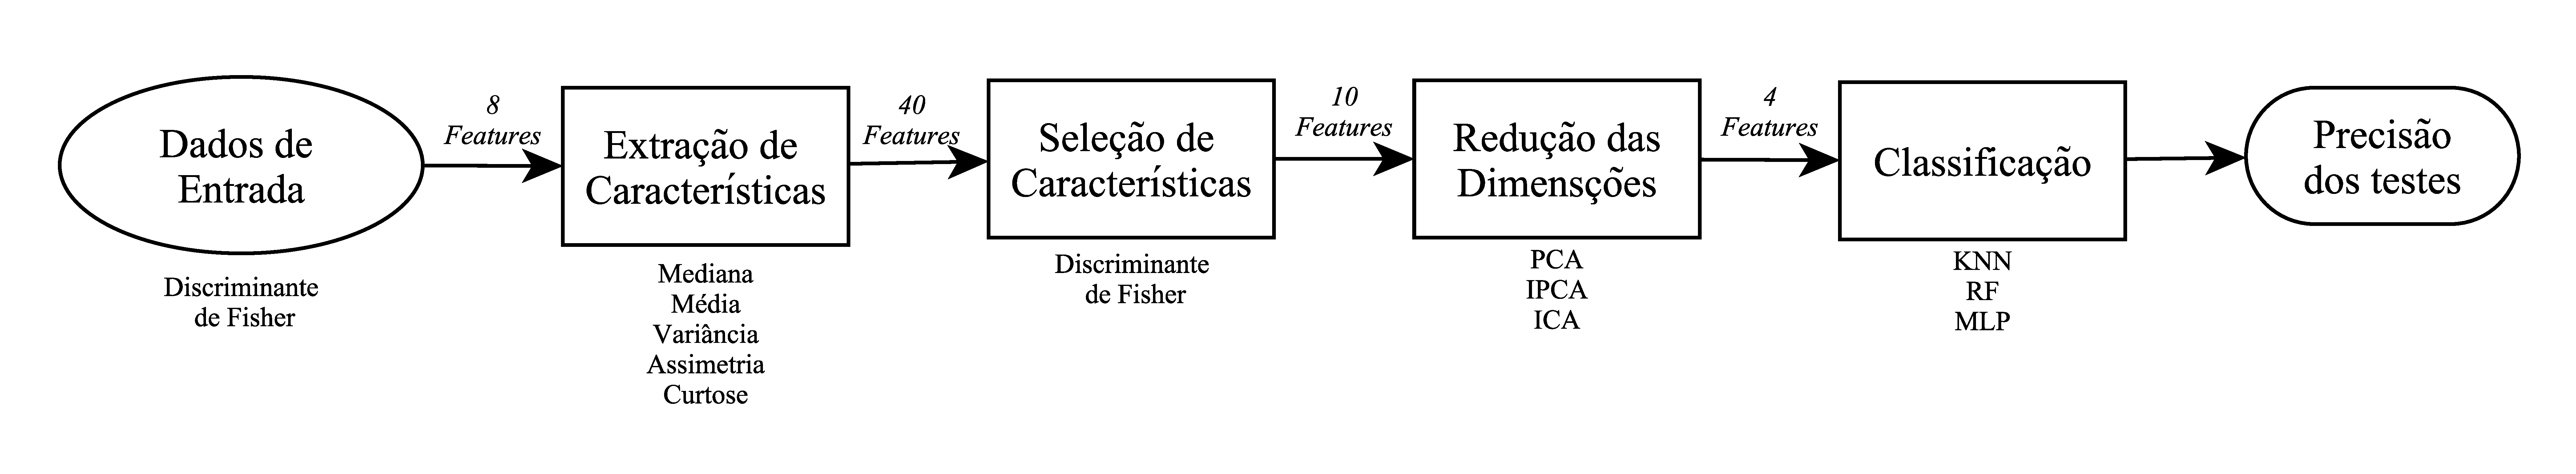
\includegraphics[width=1.\linewidth]{fluxo_projeto.eps}
	{\small Fonte: Próprio autor.} %Fonte da imagem
	\label{fig:fluxo} %rotulo para refencia
\end{figure*}


\section{Modelo Computacional Evolutivo}

Uma vez desenvolvido e testado o modelo computacional preliminar com o objetivo de comprovar a viabilidade do sistema de identificação de condutores proposto, será tomado como passo subsequente o desenvolvimento de um modelo computacional que trabalhe de modo a evoluir a medida em que o mesmo seja submetido a um fluxo de dados de direção. Para tanto, será avaliado técnicas de aprendizado de máquina \textit{online}, ou seja, que sejam capazes de se adaptar a diferentes tipos de situações e que não dependa de um novo treinamento com massa de dados.

%Em sistemas de detecção e modelagem de comportamento de condutores, este tipo de abordagem é explorada por diversos autores, pelos mesmos motivos supracitados e também pelo fato que a dinâmica de direção não ser um processo sujacente imutável. Como exemplo, \citeonline{jian2014research} utilizou filtros de Kalman  de modo a ajustar o fluxo de dados em uma janela e então os dados são submetidos a um comitê de preditores Bayesianos de forma a detectar comportamento agressivo dos condutores. Com objetivos semelhantes, \citeonline{zhang2016safety} fizeram uso de técnicas de janelamento temporal dos dados de direção, extração de caraterísticas e classificadores (Árvores de Decisão e Rede Baysiana Discreta) para a detecção de comportamento agressivo.

Muitos trabalhos que buscam realizar a modelagem de comportamento de condutores com diversas finalidades, apesar de desempenhar detecção de anomalias de forma \textit{online} \cite{jian2014research} \citeonline{zhang2016safety}, não exploram algoritmos evolutivos propriamente ditos, uma vez que somente a configuração dos classificadores parte do pressuposto que o processo subjacente é imutável. Sendo assim, serão avaliados algoritmos de aprendizado \textit{online} que tenham desempenho satisfatório à tarefa de classificação e que também sejam capazes de evoluir seu modelo a medida que novos dados são gerados. Um grupo de técnicas serão selecionadas e testadas tal que a que com o melhor desempenho e com aprendizado mais eficiente seja utilizada em implementações futuras.

\subsection{Configuração de Experimentos Futuros}

Os experimentos para avaliar o modelo de aprendizado \textit{online} serão elaborados para que os dados disponíveis nos \textit{datasets} descritos sejam submetidos no modelo computacional de forma sequencial e ordenada, simulando assim um operação direção. Assim como explorado para técnicas de aprendizado \textit{batch}, um janelamento temporal será avaliado em conjunto com técnicas de extração e seleção de características de forma  a maximizar o desempenho do classificador. Outro ponto a ser explorado é a fusão de dados de diferentes sensores complementares, como os inerciais, que estão disponíveis nos \textit{datasets} fornecidos por \citeonline{Abut2007} e \citeonline{OLIVEIRAVASCONCELOS2017}.














%\section{Desenvolvimento preliminar}
%
%Para o desenvolvimento inicial do sistema proposto, será utilizado o \textit{dataset} UYANIK, cordialmente cedido pelo VPALAB da Universidade de Sabanci (Istambul, Turquia) \cite{Abut2007}. Este \textit{dataset} contém dados de um grande número de condutores colhidos a partir de dados do barramento CAN, sensores inerciais e GPS e é amplamente utilizado em diversos trabalhos que envolvem identificação de condutores \cite{Martinez2016a} \cite{jafarnejad2017} \cite{DelCampo2014}. Estes dados servirão para avaliar a aptidão das técnicas de processamento de dados e de inteligência computacional, de modo a se determinar as que melhores se encaixam na tarefa de identificação e autenticação dos condutores.
%
%Estes resultados obtidos serão comparados com resultados quando o sistema tem como entrada os dados oriundos da interface OBD-II e sensores inerciais presentes nos \textit{smarphones}. Isto se dá uma vez que o \textit{dataset} UYANIK foi colhido por equipamentos mais sofisticados, com uma amostragem maior e menos ruidosos se comparado às fontes que serão utilizadas na aplicação final. O impacto desta diferença será avaliado no desempenho do sistema.
%
%\section{Coleta de dados}
%
%Para o desenvolvimento do sistema proposto, inicialmente será efetuada a coleta de dados que servirão como base de dados para o restante do projeto. Estes dados serão oriundos de duas fontes, a interface OBD-II (veículo) e sensores inerciais, geoposicionamento e magnéticos presentes no \textit{smartphone}.
%
%O termo OBD-II significa \textit{On-Board Diagnostics} de segunda geração. Trata-se de um sistema que, ligado à central eletrônica do carro, permite a leitura e transmissão de diversos categorias de dados, através de um dispositivo eletrônico baseado no microcontrolador ELM327, que se conecta diretamente no barramento de comunicação do veículo (normanlmente CAN-bus) efetua leituras de diversos parâmetros. De acordo com \citeonline{Abuali2016}, estas informações coletadas podem ser utilizados para análise de dados, interface com usuário e coleta de dados de sensores.
%
%Existem diversos casos na literatura que fazem uso de dados provenientes de leituras do OBD-II. Nos trabalhos de \citeonline{Martinez2015}, \citeonline{Pan2017}, \citeonline{Blaszczyk2014}, entre outros, faz-se uso de dados coletados pelo OBD-II e aplicadas técnicas de aprendizado de máquina para reconhecimento de alguns parâmetros, como agressividade, sonolência, entre outros.
%
%Cada vez mais estudos de modelagem de comportamento do condutor têm aliado ao uso de dados provenientes do OBD-II o uso de dados sensoriais originários de \textit{smartphones}. De acordo com \citeonline{Saiprasert2017}, a capacidade de multi-sensoriamento de smartphone disponíveis no mercado propicia a coleta de uma preciosa gama de dados brutos. Dados de acelerômetros fornecem uma visão do movimento longitudinal e lateral do celular, e consequentemente do veículo, enquanto o GPS nele embarcado pode fornecer dados de localização em termos de longitude e latitude.
%
%Na literatura, \textit{smartphones} têm sido empregados como ferramenta de coleta e processamento de dados em vasta gama de aplicações em sistemas veiculares. \citeonline{Hong2014} desenvolveram uma plataforma de modelagem de estilos de direção baseando-se somente em dados de sensores de \textit{smartphones}. Neste caso, os autores justificam que sistemas sensoriais para tal modelagem são caros, enquanto a penetração de mercado de \textit{smartphones} está praticamente consolidada, tendo assim aplicações desta natureza acessibilidade a praticamente todos os condutores.
%
%Ciente do potencial de aplicação destas duas fontes de dados para uso em modelagem e identificação de comportamento de condutores, pretende-se que o sistema faça a leitura do barramento CAN do veículo, baseado do aplicativo desenvolvido por \citeonline{Neto2016}. Para tal, será avaliado quais variáveis serão monitoras de acordo com a aptidão de cada uma delas em detectar padrões característicos do condutor. Como apresentado por \citeonline{jafarnejad2017}, alguns sinais têm representatividade na identificação, ângulo do volante em graus, velocidade do veículo, rotação do motor (RPM) e taxa de guinada (\textit{Yaw Rate}).
%    
%
%Para veículos brasileiros, alguns destes sinais, como o ângulo do volante, podem não estar disponíveis no mesmo. Para tal, será investigado o impacto da inexistência destes no processo e outras variáveis serão avaliadas como possíveis substitutas, de modo que a taxa de acertos do condutor seja maximizada. Não existe, porém, na literatura um consenso de quais variáveis têm maior capacidade de definir padrões que podem ser importantes na identificação do condutor.
%
%\section{Processamento de sinais}
%
%Para a aplicação de dados em qualquer técnica de aprendizado de máquina, é imprescindível que os dados sejam submetidos a um tratamento prévio, de tal modo a remover quaisquer ruídos, erros de medição e outras irregularidades nas informações.
%
%Alguns trabalhados adotaram somente um processamento estatístico básico, como o cálculo de média acumulada, desvio padrão e amplitude dos dados, como visto em \citeonline{Carmona2015}. Por outro lado, o trabalho desenvolvido por \citeonline{Kumtepe2016} representa os sinais em forma de funções de densidade de probabilidade e então modelaram-nos através de Modelo de Misturas Gaussianas (GMM). Formam-se histogramas dos dados que ainda são filtrados por meio do método das médias móveis. Segundo o autor, este método proporciona uma representação efetiva de dados de direção.
%
%Uma técnica de processamento de dados explorada por \citeonline{DelCampo2014}, especialmente para a aplicação de identificação de condutores, é a análise cepstral, aplicada como filtro e extrator de características. A técnica também é explora para processamento de sinais para identificação de condutores por \citeonline{jafarnejad2017}, em paralelo com extração estatística de características (média, mediana, curtoses, assimetria). Ambos trabalhos ressaltam que a análise cepstral é uma técnica com potencial para aplicação em identificação de condutores, por ser leve computacionalmente e adequada para futuras implementações em sistemas embarcados. Para tanto, pretende-se avaliar técnicas de pré-processamento de dados de forma a maximizar o desempenho do sistema \cite{Ahmadi-Pour2017}.
%
%
%
%\section{Algoritmo de Identificação de Condutores}
%
%Após a coleta dos dados referentes à dinâmica de direção e o processamento destes com o propósito de maximizar a extração de características, chega-se à fase de identificação do condutor por meio destes dados. Isto se dará por meio do uso de técnicas de aprendizado de máquina, em forma de classificador. Este processo será dividido em duas fases: primeiramente deve-se cadastrar o condutor autorizado a utilizar o veículo, por meio do treinamento do algoritmo. Na segunda fase, com o algoritmo já treinado para um ou mais condutores autorizados, deve-se avaliar e identificar o condutor que opera o veículo no momento.
%
%O desenvolvimento desta parte do sistema passará inicialmente pela avaliação da técnica de aprendizado de máquina mais adequada para realizar a tarefa de identificação. Para tanto, alguns requisitos serão observados:
%
%\begin{itemize}
%
%    \item \textbf{Taxa de acertos:} este parâmetro consiste em avaliar qual técnica tem melhor aptidão em identificar a autenticidade do condutor, sem que o mesmo seja avaliado como sendo autorizado quando não o é e vice-versa. Este é um ponto crítico o sistema, pois, em aplicações reais, é imprescindível que o algoritmo não cometa equívocos quanto à decisão.
%    
%    \item \textbf{Custo computacional:} tendo em vista que o \textit{hardware} a ser utilizado é limitado (\textit{smartphone}, sistemas embarcados, FPGA, entre outros), o custo computacional da técnica deve ser cuidadosamente avaliado. O tempo de treinamento do algoritmo (cadastro) é um dos principais pontos a serem avaliados neste parâmetro, pois o mesmo deve ser rápido, mas, ao mesmo tempo, eficiente, com o propósito de não comprometer o desempenho do sistema.
%    
%    \item \textbf{Tempo de processamento:} tendo em vista que o sistema deverá verificar a autenticidade do condutor, o tempo em que o algoritmo leva para efetuar tal identificação é um ponto crucial, pois, quanto mais rápido é identificado um intruso, maiores as hipóteses de se impedir a ação criminosa.
%    
%\end{itemize}
%
%No que diz respeito à \textit{driver behavior proffiling}, não existe uma unanimidade entre os autores em relação à qual técnica de aprendizado de máquina é a mais apropriada. Conforme apresentado por \citeonline{Meiring2015}, cada aplicação que envolva algum tipo de reconhecimento de padrões (distração, sonolência, embriagues, agressividade) possui uma ou mais técnicas que tiveram resultados satisfatórios. Como existem poucos trabalhos na área de identificação de condutores, ainda se tem em aberto a possibilidade de testes em diversas técnicas de aprendizado de máquina, respeitando as premissas supracitadas.
%
%Serão selecionados diversos algoritmos de classificação, dos quais serão avaliados o desempenho, de acordo com os requisitos definidos. Das técnicas que serão testadas, selecionou-se algumas que obtiveram desempenho satisfatório em outros trabalhos relacionados à identificação de condutores, dentre os quais pode-se citar:
%
%\begin{itemize}
%    \item \textbf{AdaBoost}, utilizado por \citeonline{jafarnejad2017}.
%    
%    \item \textbf{Gradient Boosting}, utilizado por \citeonline{jafarnejad2017}.
%    
%    \item \textbf{Extra Trees}, utilizado por \citeonline{jafarnejad2017}.
%    
%    \item \textbf{\textit{Extreme Learning Machines}}, utilizado por \citeonline{Martinez2016a}.
%    
%    
%    \item \textbf{Máquinas de Vetor de Suporte}, utilizado por \citeonline{Chen2015} e \citeonline{jafarnejad2017}.
%    
%    \item \textbf{Redes Neurais Artificiais}, utilizado por \citeonline{DelCampo2014}.
%    
%    \item \textbf{Florestas Aleatórias}, utilizado por \citeonline{Wang2017a} e \citeonline{jafarnejad2017}.
%
%\end{itemize}
%
%É importante salientar que outros algoritmos ainda não utilizados em outros projetos poderão ser testados, uma vez identificada sua capacidade de desempenhar a tarefa de identificação e autenticação de condutores.
%
%\section{Desenvolvimento de aplicação móvel Android}
%
%Todos os elementos citados anteriormente irão compor um aplicativo para sistema operacional Android, que irá desempenhar a tarefa de identificação de condutores. Para isto, o desenvolvimento do mesmo irá se basear no trabalho desenvolvido por \citeonline{Neto2016}, que consiste basicamente num aplicativo que efetua leituras do dispositivo OBD-II, por meio da interface \textit{Bluetooth}, e também recolhe informações de sensores presentes no \textit{smartphone}, tais como acelerômetro, giroscópio, bússola (sensor de orientação) e GPS.
%
%Diversos trabalhos exploram aplicações baseadas em Android, para a realização da tarefa de modelagem do perfil de condutores. Isto se deve muito à capacidade computacional que os \textit{smartphones} possuem atualmente, aliado à aptidão que os sensores presentes nos mesmos têm de realizar leitura da dinâmica de direção como um todo.
%
%Como exemplo, o aplicativo \textit{DrivingStyles} desenvolvido por \citeonline{Meseguer2017}, que, através destas leituras, utiliza uma rede neural artificial treinada que identifica o estilo de direção do condutor entre calmo, normal e agressivo. De forma semelhante, \citeonline{Saiprasert2017} desenvolveram um aplicativo que monitora toda a dinâmica de direção e indica possíveis comportamentos que possam ser perigosos aos usuários do veículo.
%
%Sendo assim, o uso de aplicativos móveis é uma ferramenta poderosa para implementação de sistemas que abranjam identificação de comportamento de condutores através de sensores que monitorem a dinâmica de direção. Portanto, para o presente trabalho, o desenvolvimento de um aplicativo que embarque todos os elementos que serão desenvolvidos é uma forma interessante de validar o sistema de uma maneira simples, eficiente e acessível a um custo relativamente baixo.